
{
    The Bag of Tricks\cite{Luo_2019_CVPR_Workshops} model is a vital component of contemporary appearance-based object tracking. 
    It finds application in Strong SORT and Deep OC-SORT, highlighting its significance in state-of-the-art tracking algorithms; 
    this is also the reason to use \ac{BoT} within this project. 
}

{
    \ac{BoT} is a composed by a backbone module and a neck. 
    The last layer from the backbone before the backbone task realization (on a classification head) is extracted as features for the \ac{BoT} neck. 
    Within the \ac{BoT} neck there is a sequence of operations consisting in: a batch normalization layer, its output is the appearance metric output, and a generalized mean pooling layer, its output is a classification output. 
%    A block diagram of \ac{BoT} is shown in Figure \ref{fig:bot_diagram}.
}

{
    The backbone used is the residual network of 50 layers (ResNet50) with non-local blocks. 
    This choice of architecture empowers the model with the ability to capture intricate spatial dependencies and semantic information. 
}

{
    A more comprehensive exploration of the project-specific considerations will be presented in the methodology section.
}

%\begin{figure}[!tb]
%    \centering
%    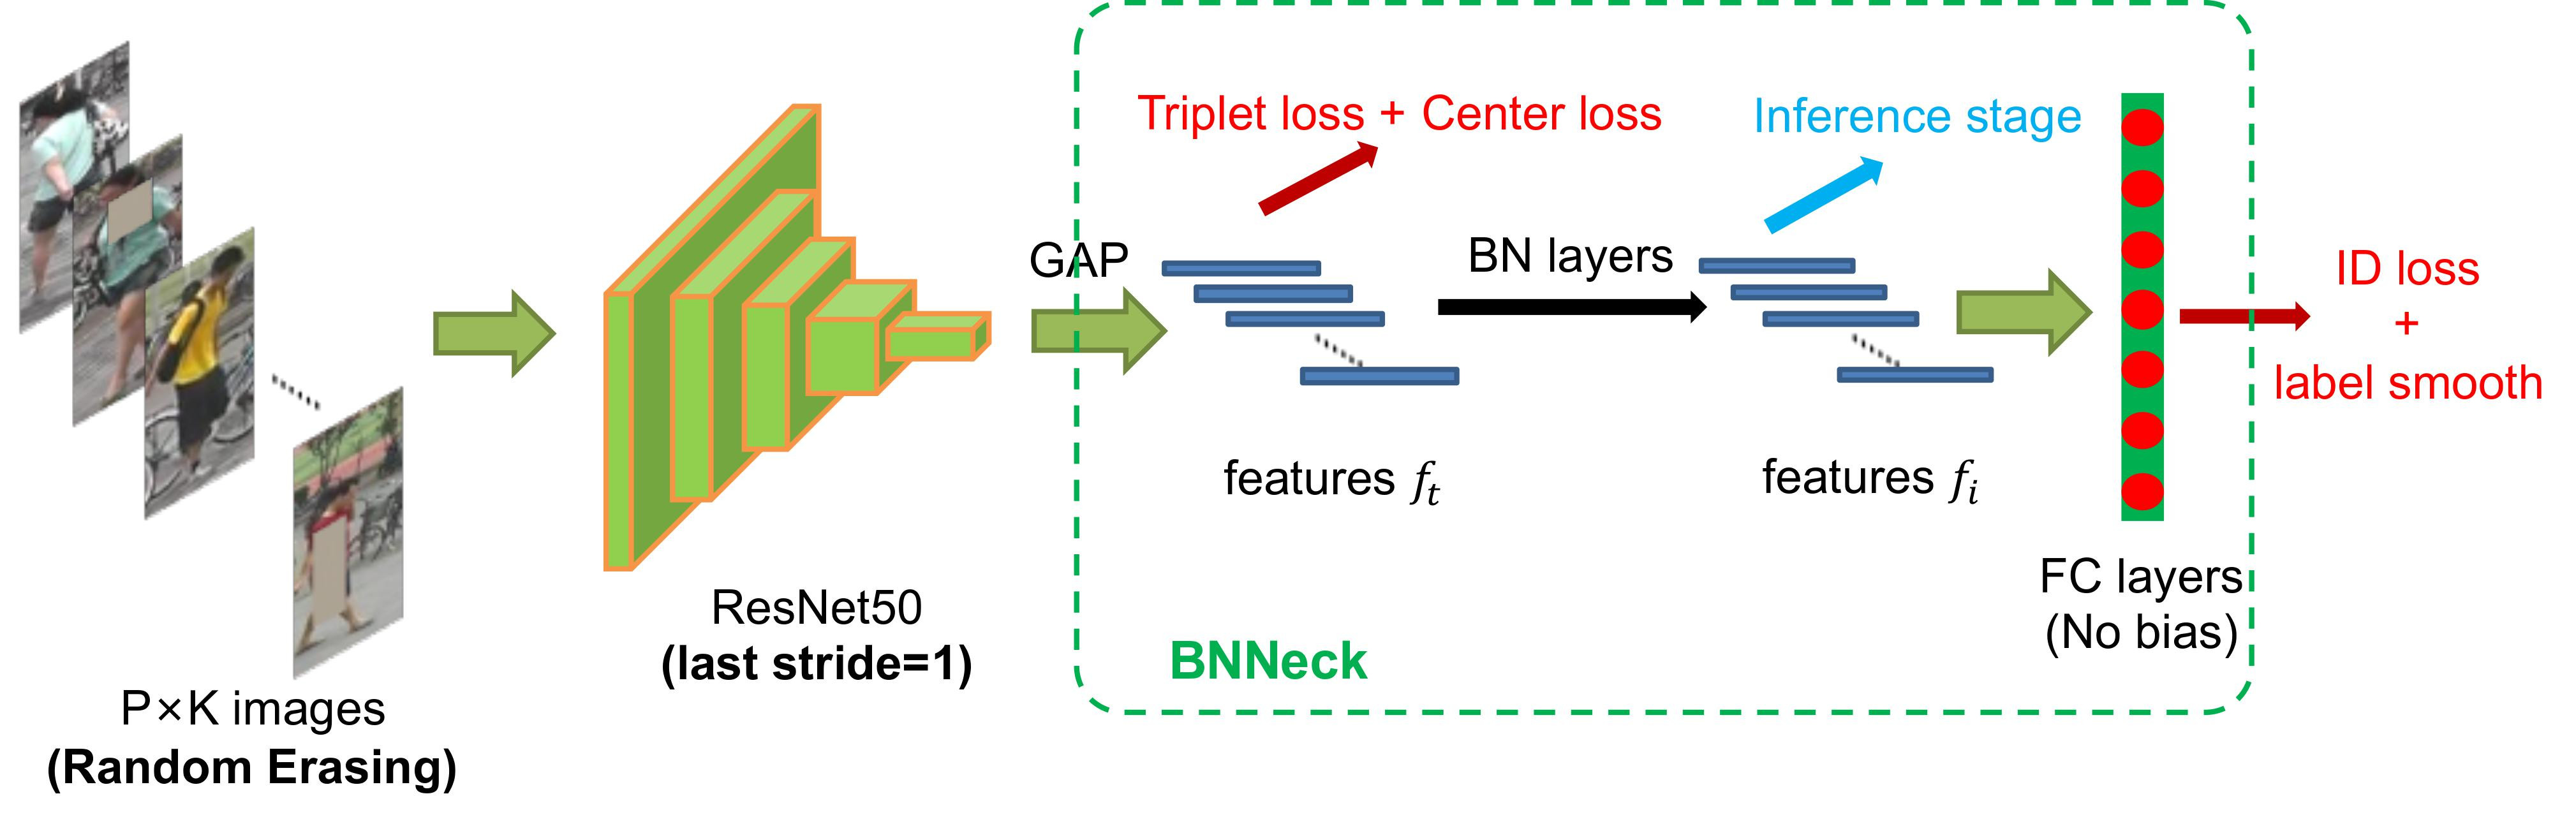
\includegraphics[width=0.8\linewidth]{figures/05_methodology/BagOfTricksBlokDiagram.jpg}
%    \caption[Bag of Tricks model block diagram]{\footnotesize{
%            Block diagram of the Bag of Tricks model from the Bag of Tricks paper\cite{Luo_2019_CVPR_Workshops}.
%        }}
%    \label{fig:bot_diagram}
%\end{figure}
